\section{Pipeline}

Surface Reconstruction from Point Sets is a sequential process:

\begin{itemize}
\item Scanning and scan alignment produce a set of points
      or points with normals. Alignment is not yet
      covered by \cgal.
\item Outlier removal for reconstruction methods which
      are not resilient to outliers.
\item Simplification to reduce the number of input points.
\item Smoothing to reduce noise in the input data.
\item Normal estimation and orientation when the normals
      are not already provided by the acquisition device.
\item Surface reconstruction.
\end{itemize}

\cgal\ provides algorithms for all steps listed above except alignment.\\
Chapter \ccc{Point_set_processing_3} \ref{chap:point_set_processing_3} describes outlier removal, simplification, smoothing,
normal estimation and orientation.\\
This package provides surface reconstruction using \cgal\ Surface Mesh Generator.

A demo running on Windows is currently provided,
and will be replaced soon by a complete point set demo based on QT4 and QGlViewer.
It features all steps listed above except alignment.

% Insert image pipeline.jpg/eps
\begin{center}
    \label{Surface_reconstruction_points_3-fig-pipeline}
    % Image
    \begin{ccTexOnly}
        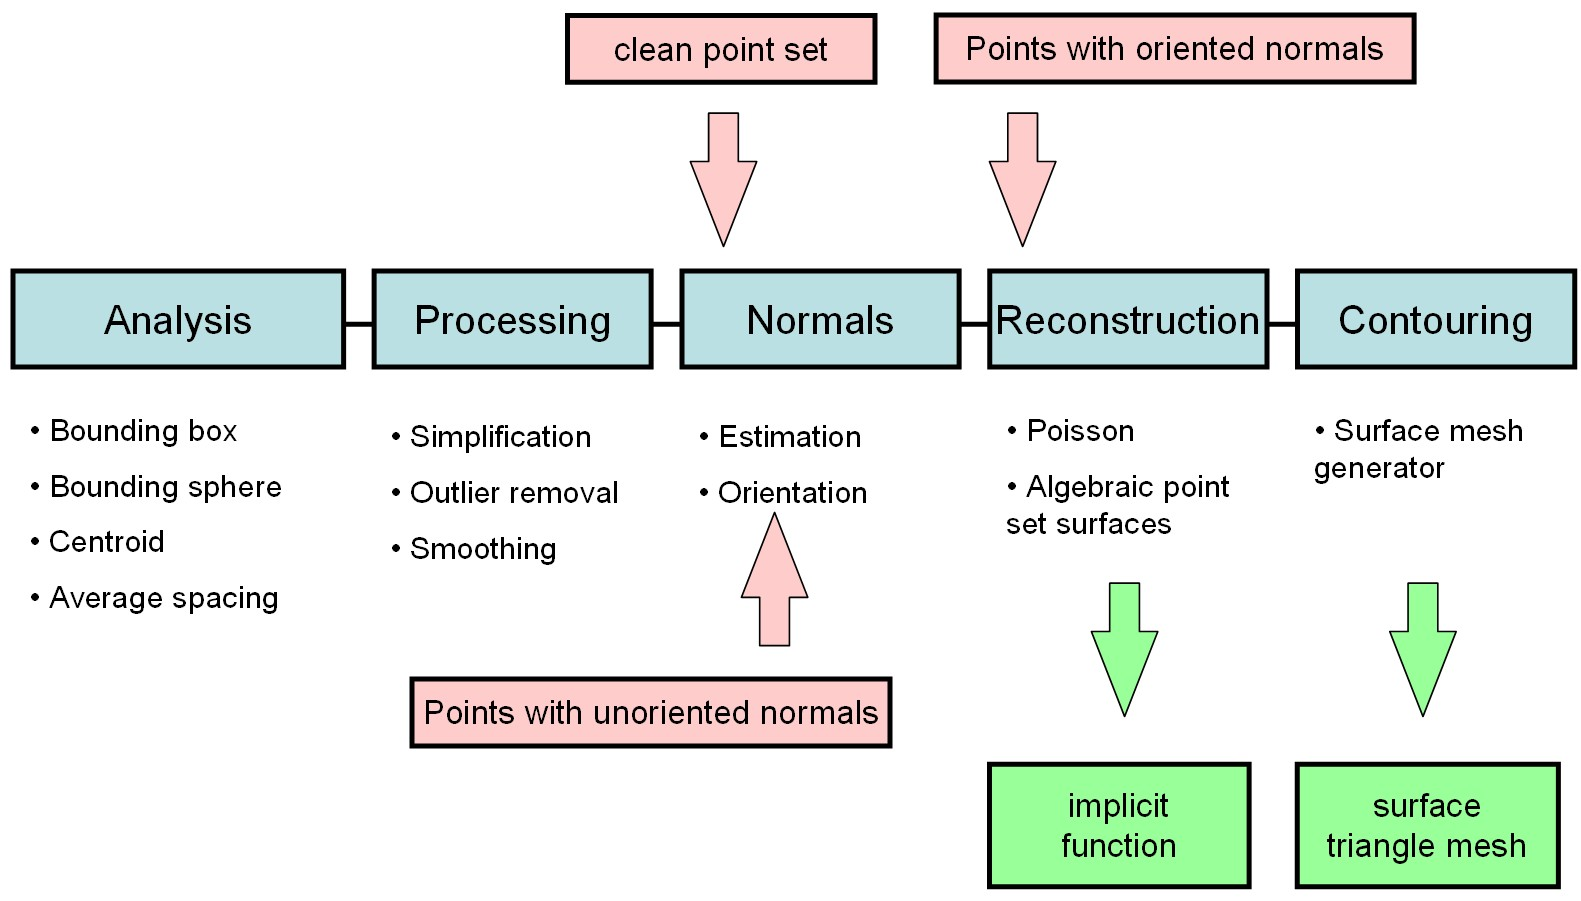
\includegraphics[width=1.0\textwidth]{Surface_reconstruction_points_3/pipeline} % omit .eps suffix
    \end{ccTexOnly}
    \begin{ccHtmlOnly}
        <img width="70%" border=0 src="./pipeline.jpg"><P>
    \end{ccHtmlOnly}
    % Title
    \begin{figure}[h]
        \caption{Surface Reconstruction from Point Sets pipeline.}
    \end{figure}
\end{center}


\subsection{Input and Preprocessing}

This component expect as input parameters range iterators over 3D points with oriented normals.

See Chapter \ccc{Point_set_processing_3} \ref{chap:point_set_processing_3} to read point sets from files and preprocess them.


\subsection{Surface Reconstruction}

The two surface reconstruction methods fall into the category of the implicit surface reconstruction approaches in the sense that they both compute a scalar function whose iso-surface approximates the input oriented points.
\begin{itemize}
\item Delaunay-based Poisson reconstruction inspired
      from \cite{Kazhdan06}. This method solves for
      an approximate indicator function of the inferred
      solid. The solving stage must be done once for all
      before iso-contouring. % refer to basics?
\item Algebraic point set surfaces \cite{Guennebaud07}.
      This method falls into the category of so-called
      point set surfaces, where the approximate
      signed distance function to the inferred surface
      can be evaluated at any query point, on the fly
      during iso-contouring.
\end{itemize}

\ccRefIdfierPage{CGAL::Poisson_reconstruction_function<GeomTraits, ReconstructionTriangulation_3>}  \\
\ccRefIdfierPage{CGAL::APSS_reconstruction_function<GeomTraits>}  \\

% Insert image APSS.jpg/eps
\begin{center}
    \label{Surface_reconstruction_points_3-fig-APSS}
    % Image
    \begin{ccTexOnly}
        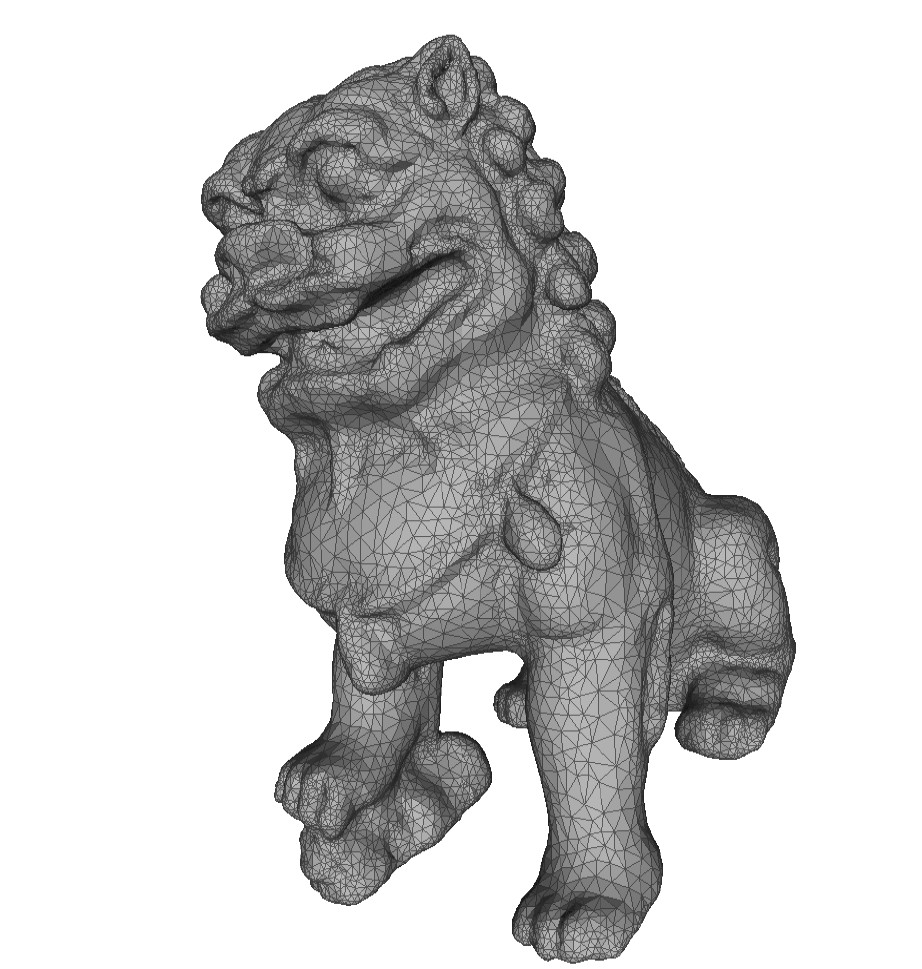
\includegraphics[width=0.5\textwidth]{Surface_reconstruction_points_3/APSS} % omit .eps suffix
    \end{ccTexOnly}
    \begin{ccHtmlOnly}
        <img width="50%" border=0 src="./APSS.jpg"><P>
    \end{ccHtmlOnly}
    % Title
    \begin{figure}[h]
        \caption{APSS surface reconstruction from 10K
                 points sampled with a Minolta laser scanner.}
        % later: add computed function
    \end{figure}
\end{center}

The computed implicit functions can be iso-contoured to reconstruct a surface by using the \cgal\ surface mesh generator~\cite{cgal:ry-gsddrm-06,cgal:bo-pgsms-05}.

\ccRefIdfierPage{CGAL::make_surface_mesh}  \\

The parameter \ccc{Tag} affects the behavior of \ccc{make_surface_mesh()}: \\
- \ccc{Manifold_tag}: the output mesh is guaranteed to be a manifold surface without boundary.\\
- \ccc{Manifold_with_boundary_tag}: the output mesh is guaranteed to be manifold and may have boundaries.\\
- \ccc{Non_manifold_tag}: the output mesh has no guarantee and hence is outputted as a polygon soup.

Example:
See \ccc{poisson_reconstruction_example.cpp} example above.


\subsection{Output}

The surface reconstructed by \ccc{make_surface_mesh()} is required to be a model of the concept \ccc{SurfaceMeshComplex_2InTriangulation_3}, a data structure devised to represent a two dimensional complex embedded into a three dimensional triangulation.\\

\ccc{SurfaceMeshComplex_2InTriangulation_3} defines the methods to traverse the reconstructed surface.

As examples, we provide functions to:

\begin{itemize}
\item Write the reconstructed surface mesh to the
      OFF file format.
\item Convert the reconstructed surface mesh to a
      polygon soup.
\end{itemize}

\ccRefIdfierPage{CGAL::output_surface_facets_to_off}  \\
\ccRefIdfierPage{CGAL::surface_reconstruction_output_surface_facets}  \\

Example:

See \ccc{poisson_reconstruction_example.cpp} example above.
